\section{Problem 8}

\subsection{Code}

\begin{lstlisting}
function [pZ_H0,pZ_H1,lambda0,Pd,ZVec] = performAcqHypothesisCalcs(s)
% performAcqHypothesisCalcs : Calculate the null-hypothesis and alternative
%                             hypothesis probability density functions and 
%                             the decision threshold corresponding to GNSS 
%                             signal acquisition with the given inputs.
%
% Z is the acquisition statistic:
%
%        N  |    |^2
% Z =   sum | Sk |
%       k=1 |    |
%
%
%
%      N   |             |
%   = sum  | Ik^2 + Qk^2 |
%     k=1  |             |
%
%
%
% where Sk = rhok + nk = Ik + j*Qk
%
% and nk = nIk + j*nQk
%
% with nIk ~ N(0,1), nQk ~ N(0,1), and E[nIk nQi] = 1 for k = i and 0 for k !=
% i. The amplitude rhok is related to familiar parameters Nk, Abark, and
% sigma_IQ by rhok = (Nk*Abark)/(2*sigma_IQ), i.e., it is the magnitude of the
% usual complex baseband phasor normalized by sigma_IQ.
%
% Under H0, the statistic Z is distributed as a chi square distribution with
% 2*N degrees of freedom; under H1, it is distributed as a noncentral chi
% square distribution with lambda = N*rhok^2 and 2*N degrees of freedom.
%
% The total number of cells in the search grid is assumed to be nCells =
% nCodeOffsets*nFreqOffsets, where nFreqOffsets = 2*fMax*Ta and Ta = Na*T is
% the total coherent accumulation time. Here, Na is the average value of the
% number of samples in each accumulation, Nk.
%
% INPUTS
%
% s -------- A structure containing the following fields:
%
% C_N0dBHz ------- Carrier to noise ratio in dB-Hz.
%
% Ta ------------- Coherent accumulation interval, in seconds.
%
% N -------------- The number of accumulations summed noncoherently to
%                  get Z.
%
% fMax ----------- Frequency search range delimiter. The total
%                  frequency search range is +/- fMax.
%
% nCodeOffsets --- Number of statistically independent code offsets in
%                  the search range.
%
% PfaAcq --------- The total acquisition false alarm probability.
%                  This is the probability that the statistic Z
%                  exceeds the threshold lambda in any one of the
%                  search cells under the hypothesis H0. One can
%                  derive the false alarm probability for *each*
%                  search cell from PfaAcq. This procedure is
%                  straightforward if we assume that the detection
%                  statistics from the search cells are independent
%                  of one another.
%
% ZMax ----------- The maximum value of Z that will be considered.
%
% delZ ----------- The discretization interval used for the
%                 independent variable Z. The full vector of Z
%                 values considered is thus ZVec = [0:delZ:ZMax].
%
%
% OUTPUTS
%
% pZ_H0 ---------- The probability density of Z under hypothesis H0.
%
% pZ_H1 ---------- The probability density of Z under hypothesis H1.
%
% lambda0 -------- The detection threshold.
%
% Pd ------------- The probability of detection.
%
% Zvec ----------- The vector of Z values considered.
%
%+------------------------------------------------------------------------+
% References:
%
%
%+========================================================================+
dof = 2*s.N;
ZVec = 0:s.delZ:s.ZMax;
nFreqOffsets = 2*s.fMax*s.Ta;
nCells = s.nCodeOffsets * nFreqOffsets;
rho_squared = 10^(s.C_N0dBHz/10) * 2 * s.Ta;
lambda = s.N * rho_squared;

% compute the probability density of Z under hypothesis H0 and H1
pZ_H0 = chi2pdf(ZVec, dof)';
pZ_H1 = ncx2pdf(ZVec, dof, lambda)';

% Calculate the threshold that ensures that the probability of false 
% acquisition is below the user-defined value
Pf = 1 - (nthroot((1-s.PfaAcq), nCells));
nuStar = chi2inv(1-Pf, dof);
lambda0 = nuStar;

% Calculate the probability of detection
Pd = 1 - ncx2cdf(nuStar, dof, lambda);
\end{lstlisting}


\subsection{Results}

\subsubsection{Part A}

In part A, N was adjusted to reach a probability of detection in the neighborhood
of 95\% for signals with different carrier-to-noise ratios, this is shown in
Figure~\ref{fig:pd_vs_N}.

\begin{figure}[H]
	\centering
	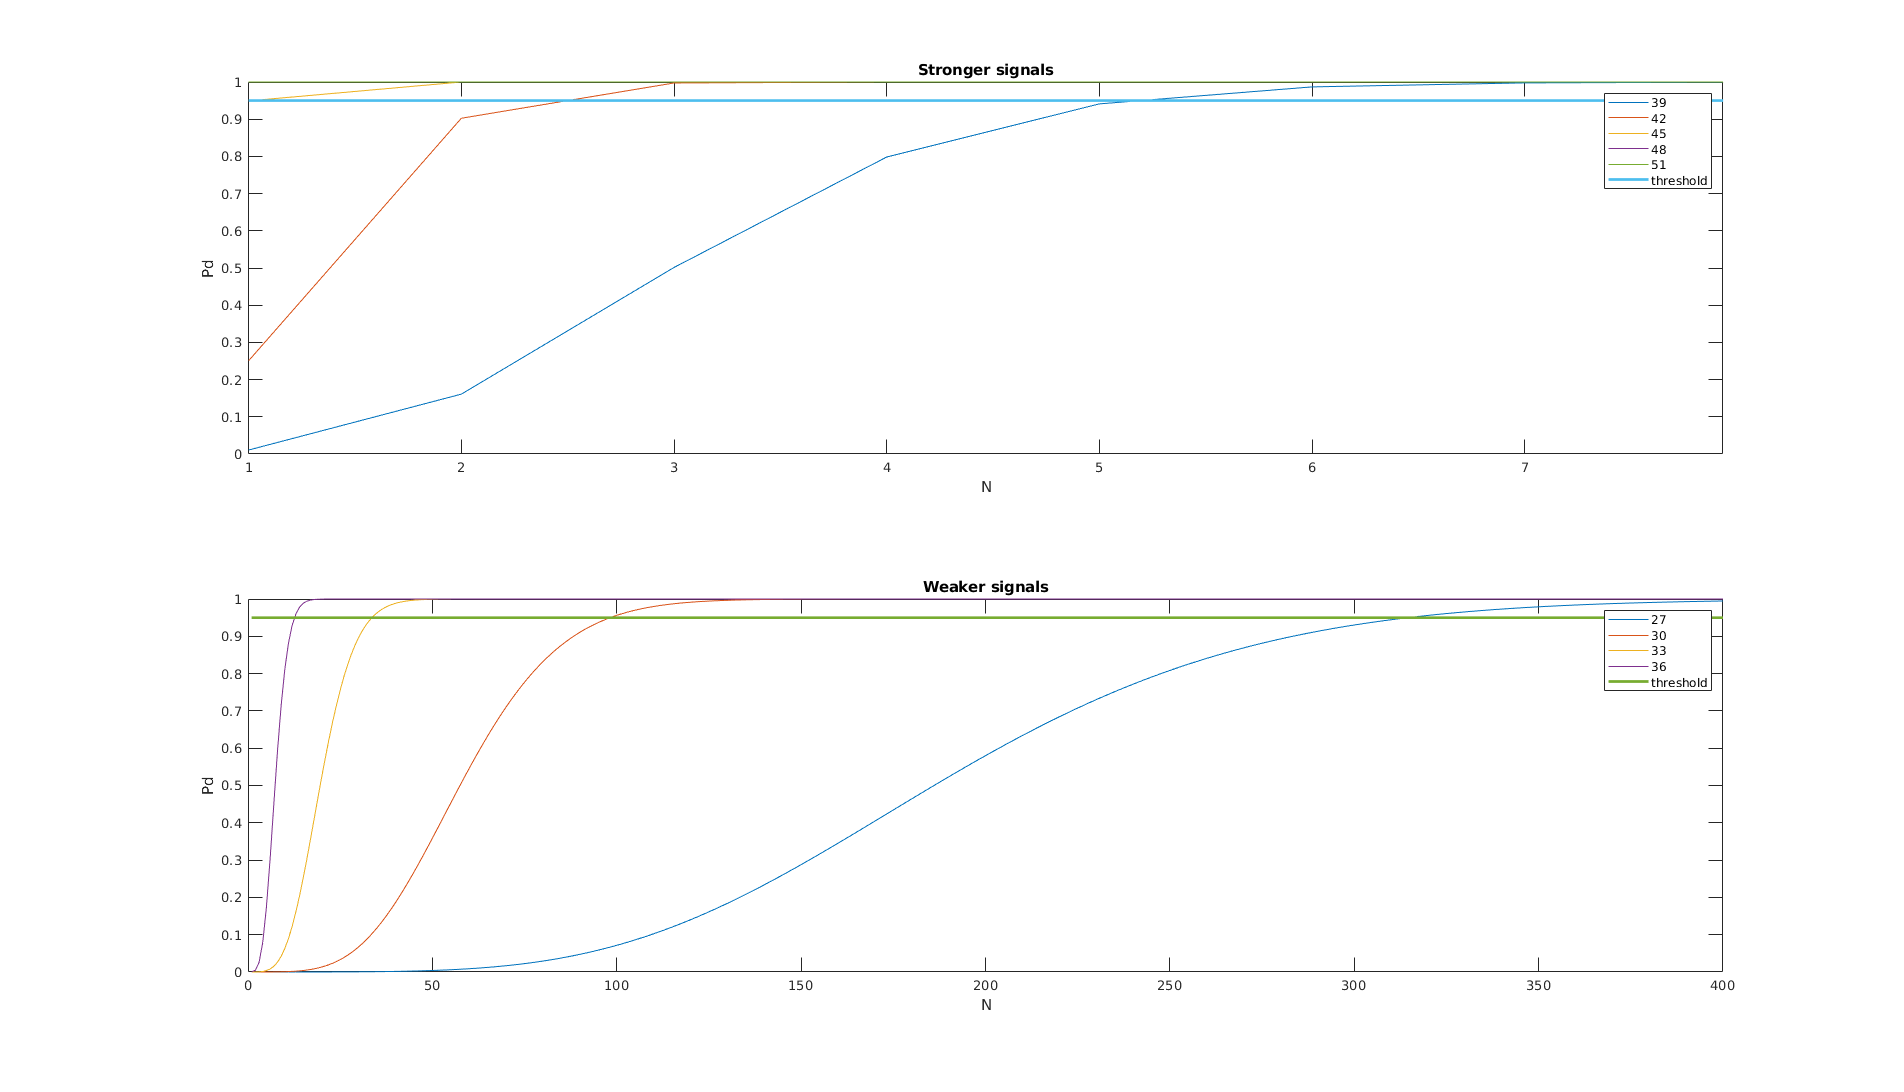
\includegraphics[width=0.9\textwidth]{figs/Pd_vs_N.png}
	\caption{Probability of detection vs. number of accumulation periods for
		different C/N0 ratios (Non-coherent accumulation).}
	\label{fig:pd_vs_N}
\end{figure}

In Figure~\ref{fig:HT_partA_30dBHz} it is possible to observe a particular case
of the hypothesis testing for GNSS acquisition. In particular, it is taylored
to detect a 30dBHz C/N0 signal with 95\% probability and 0.01\% chance of false
alarm by performing non-coherent integration.

\begin{figure}[H]
	\centering
	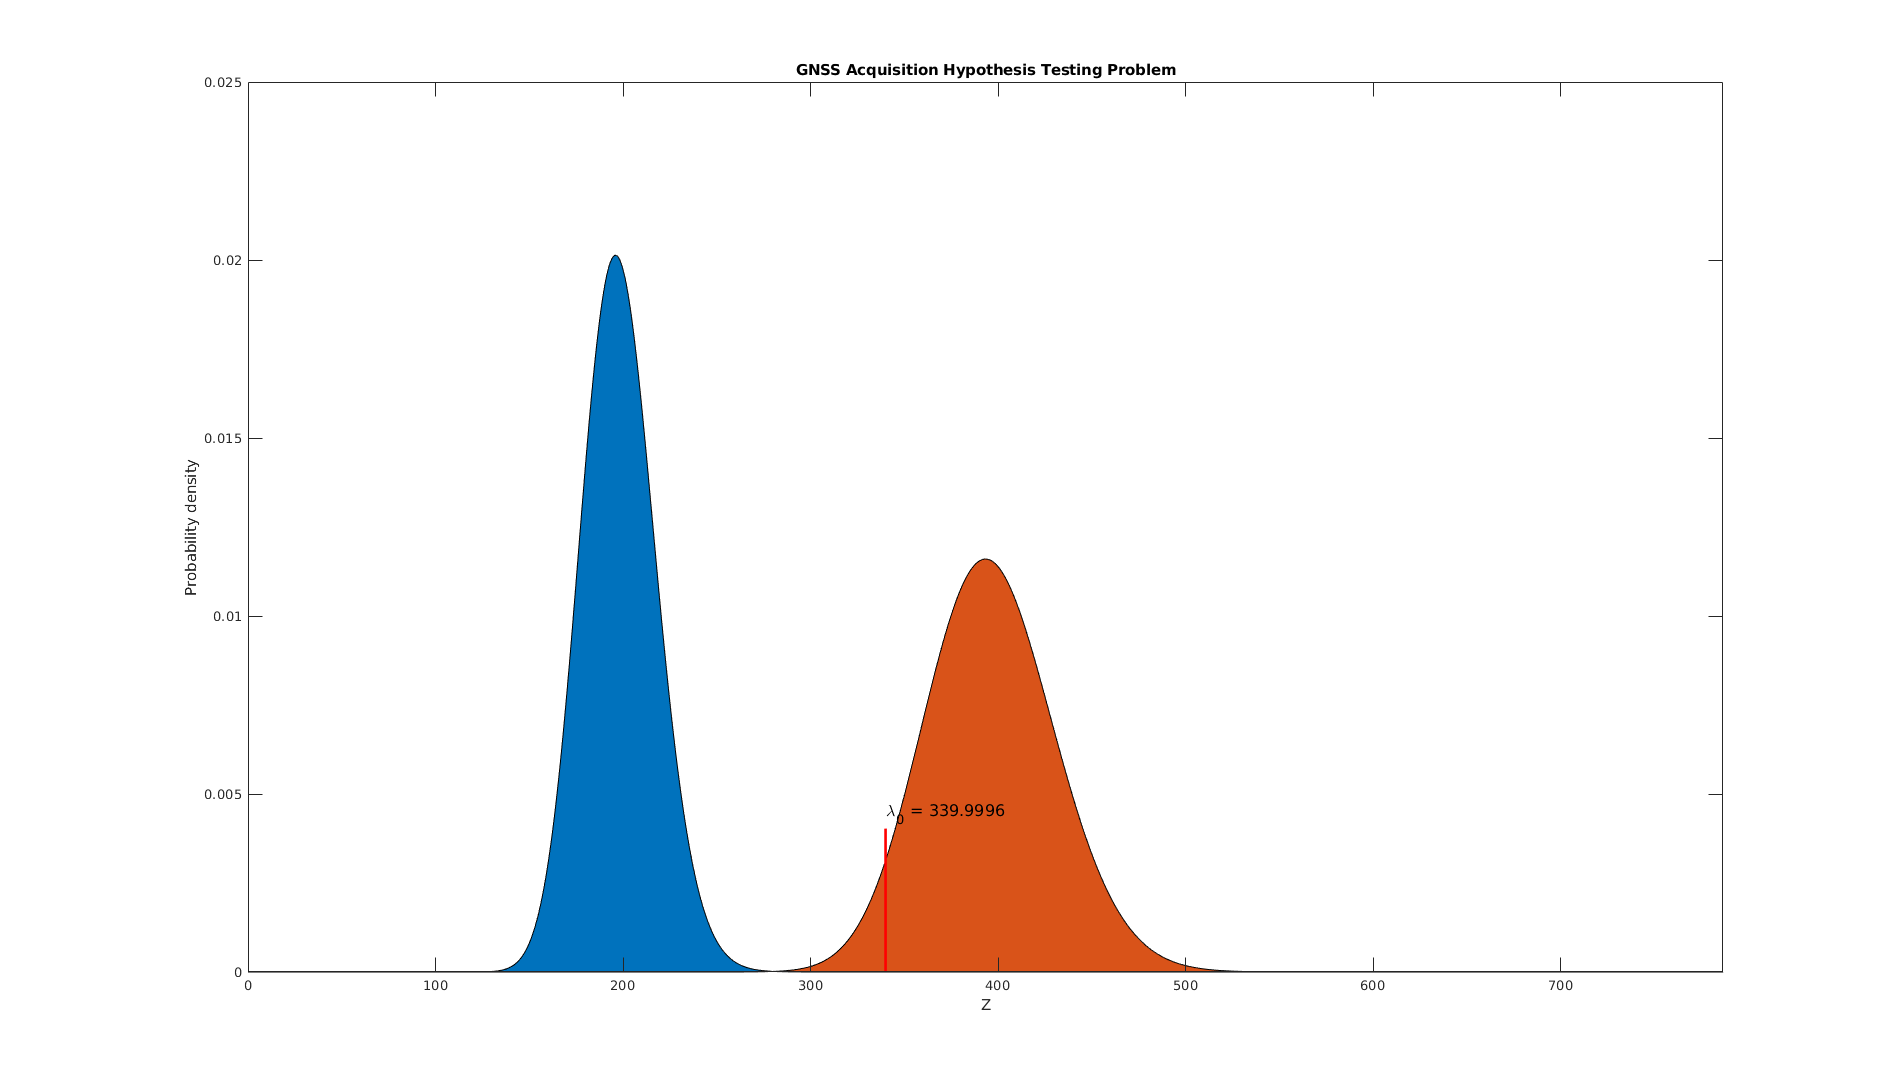
\includegraphics[width=0.9\textwidth]{figs/HT_partA_30dBHz.png}
	\caption{Hypothesis testing for the case where a 30dBHz carrier to noise ratio
		signal. The detection threshold was set to have a probability of false alarm
		0.0001. Then, using $Ta=1ms$, N was adjusted to get a probability of detection
		greater than 95\%. Thus, $N=99$.}
	\label{fig:HT_partA_30dBHz}
\end{figure}

\subsubsection{Part B}

In part B, Ta was adjusted to reach a probability of detection in the neighborhood
of 95\% for signals with different carrier-to-noise ratios, this is shown in
Figure~\ref{fig:pd_vs_Ta}.

\begin{figure}[H]
	\centering
	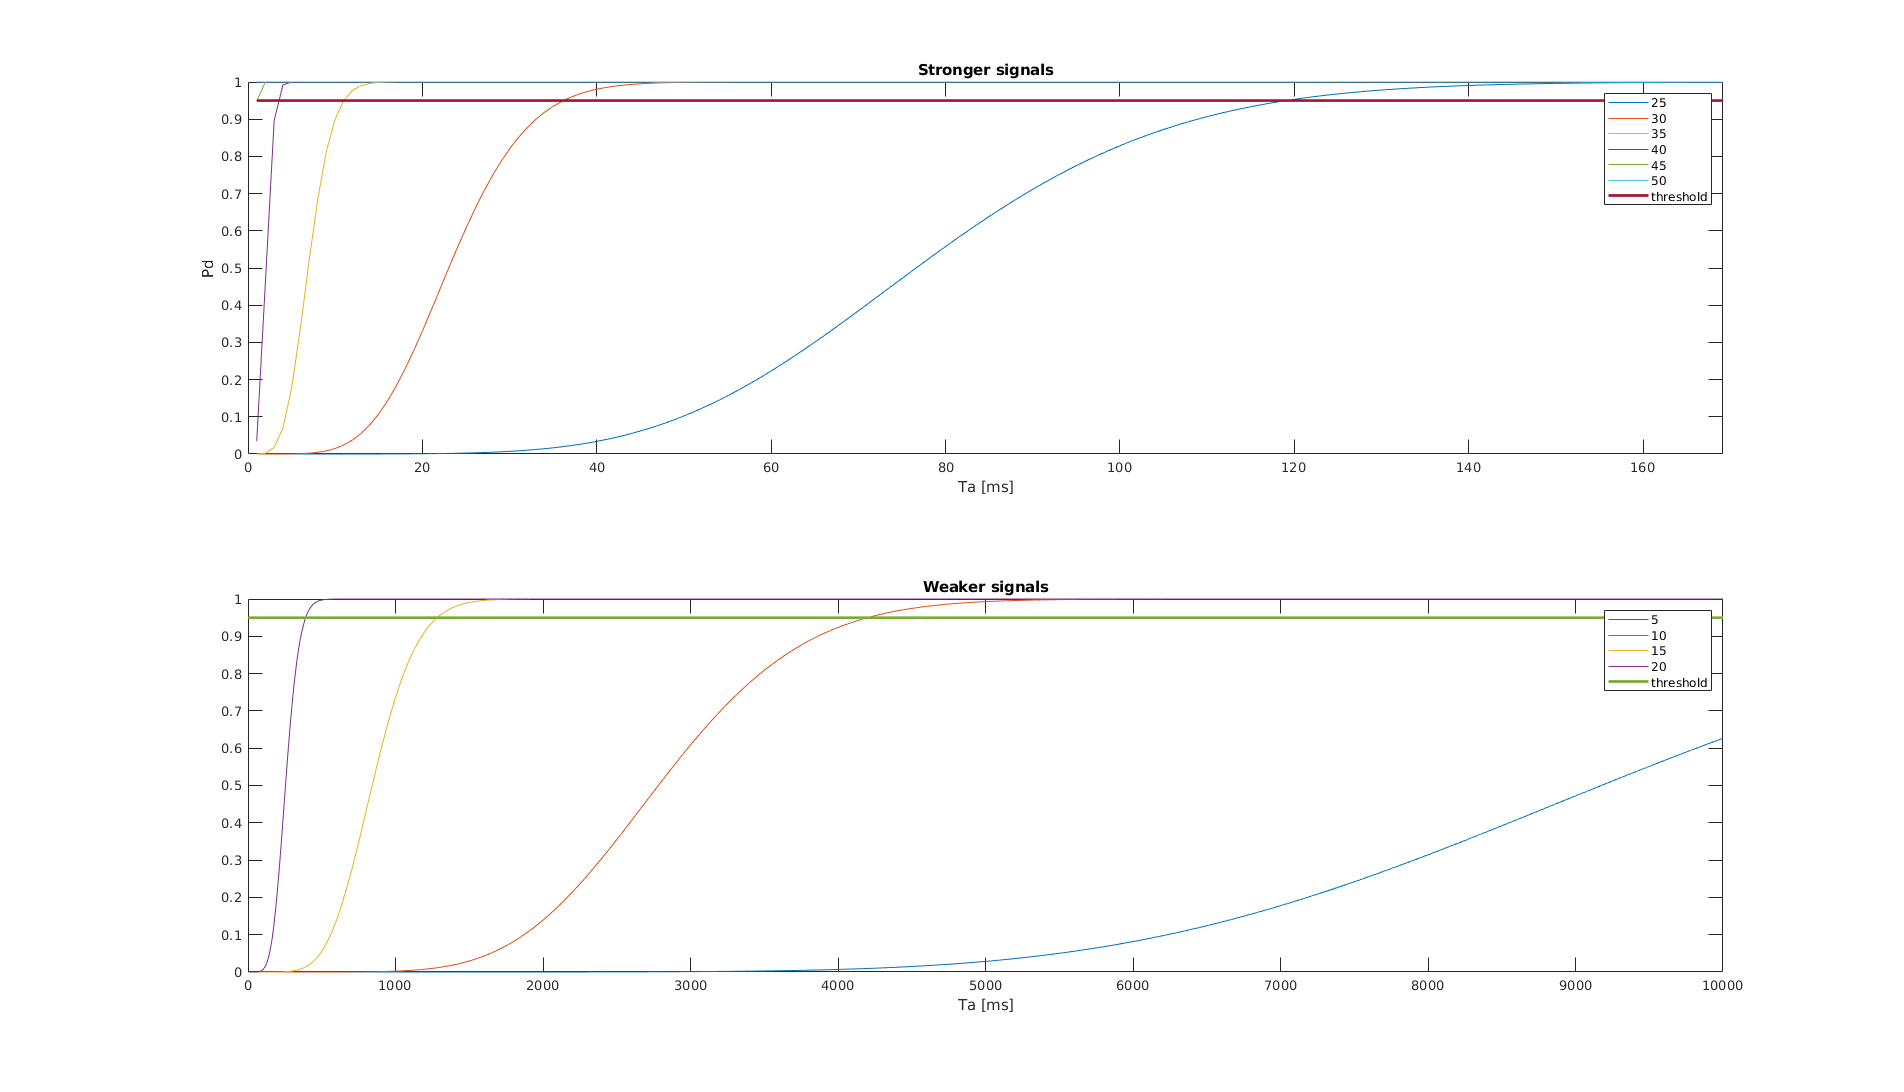
\includegraphics[width=0.9\textwidth]{figs/Pd_vs_Ta.png}
	\caption{Probability of detection vs. accumulation period for
		different C/N0 ratios (Coherent accumulation).}
	\label{fig:pd_vs_Ta}
\end{figure}

In Figure~\ref{fig:HT_partB_30dBHz} it is possible to observe a particular case
of the hypothesis testing for GNSS acquisition. In particular, it is taylored
to detect a 30dBHz C/N0 signal with 95\% probability and 0.01\% chance of false
alarm by performing coherent integration.

\begin{figure}[H]
	\centering
	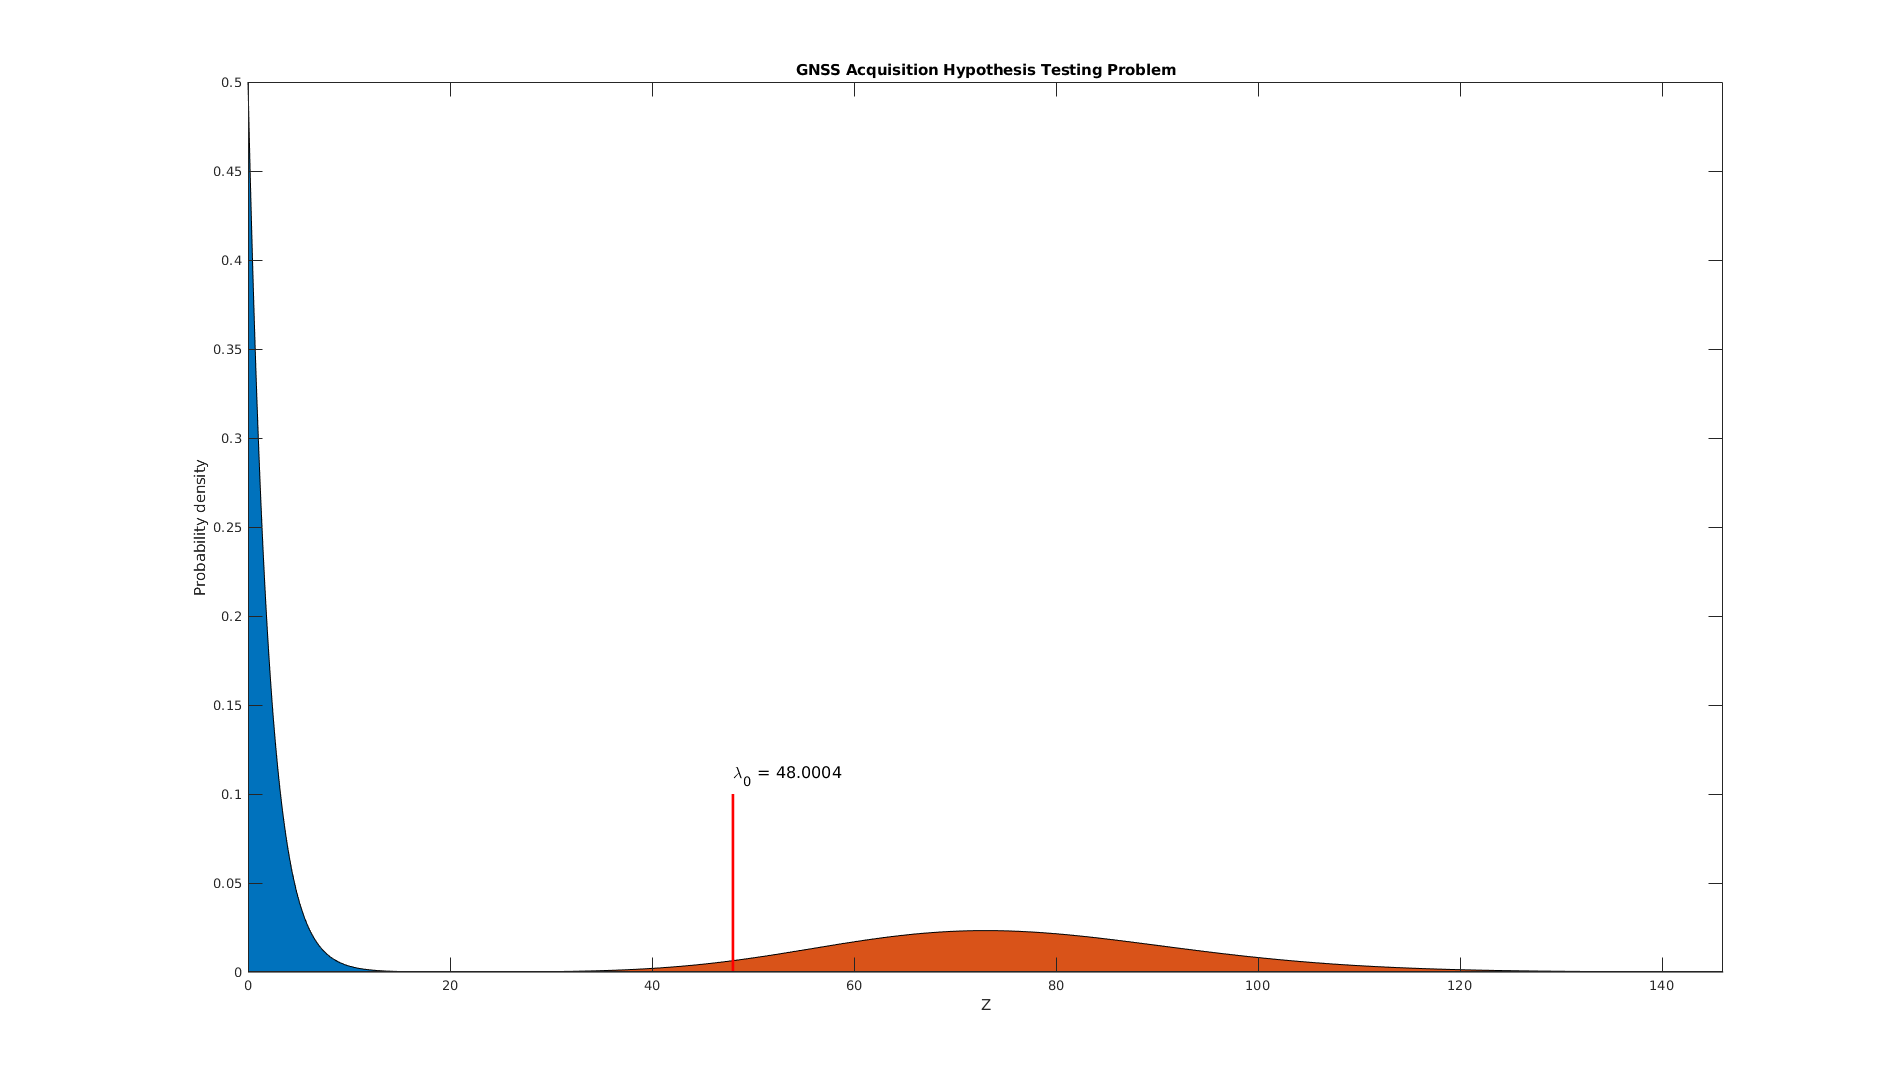
\includegraphics[width=0.9\textwidth]{figs/HT_partB_30dBHz.png}
	\caption{Hypothesis testing for the case where a 30dBHz carrier to noise ratio
		signal. The detection threshold was set to have a probability of false alarm
		0.0001. Then, using $N=1$, $Ta$ was adjusted to get a probability of detection
		greater than 95\%. Thus, $Ta=37ms$.}
	\label{fig:HT_partB_30dBHz}
\end{figure}


Analizing Figure~\ref{fig:HT_partA_30dBHz} and \ref{fig:HT_partB_30dBHz} its is
possible to see that coherent integration leads to a lower overall data usage.
since it needs 37ms of the signal while the non-coherent integration need to
process 99 intervals of 1ms each.
